\section{Программная реализация модуля «НейроКОМПАС-3D»}

TODO2

\subsection{Дата-инженерный контур и пайплайн обучения}

\begin{enumerate}
    \item в качестве сырого датасета используется папка, содержащая вложенные папки произвольного числа уровней вложенности, заканчивающиеся папками моделей, внутри которых лежат файлы вида \{model\_name\}index\{i1\}.stl, \{model\_name\}index\{i1\}.stp, \{model\_name\}index\{i2\}.stl, \{model\_name\}index\{i2\}.stp, \{\ldots\}, \{model\_name\}.json;
    \item вызывается скрипт, преобразующий данный датасет в промежуточный вид “Step0.stp”, “Step1.stp”, \ldots “Steps.txt”, внутри которого можно контролировать, какие операции разрешается и запрещается оставлять в датасете, какие ограничения накладываются на типы и сложность контуров;
    \item вызывается скрипт, преобразующий промежуточный формат в итоговый, пригодный напрямую для использования MeshCNN, использующий STEP файлы и Steps.txt для автоматической разметки моделей (раскраски рёбер в соответствии с порождающей операцией) и конвертацией их в OBJ файлы, с возможностью контролировать тип операции, тип задачи (классификация / сегментация), ограничения на сложность конечной модели;
    \item в результате предыдущих шагов получается датасет в виде папки datasets/generated/, с вложенными папками: train/ (содержащим сгенерированные OBJ файлы), seg/ и sseg/ (содержащие файлы с информацией об образцовой разметке типов рёбер);
    \item копируется часть файлов из папки train/ в test/ для создания тестовой выборки для валидации обучаемости модели (обычно 10\%);
    \item вызывается обучение, следить за процессом которого можно с помощью утилиты tensorboard;
    \item результаты обучения записываются в папку checkpoints/generated, из которых можно брать веса обученной нейронной сети в формате .pth.
\end{enumerate}



\subsection{Контур инференса и исполняемый модуль main.exe}

\begin{enumerate}
    \item программный код получает на вход единый STEP файл некой 3D модели, которую пользователь хочет “упростить” --- получить дерево построения;
    \item триангулирует STEP файл с неким deflection, преобразуя его в STL файл для дальнейшей работы, где deflection подбирается бинарным поиском с целью получить максимальное число треугольников, но не превышающее 1500;
    \item STL файл преобразуется в OBJ, где вершины на расстоянии меньше $10^{-5}$ объединяются, рёбра не повторяются, грани с нулевой площадью удаляются;
    \item подготавливается папка для запуска MeshCNN: создаются папки train, test, seg, sseg; полученный OBJ файл помещается в папки train и test, в seg и sseg помещаются мок-файлы, зависящие только от числа рёбер в исходной модели;
    \item запускается MeshCNN, который в том числе производит нормализацию модели, и автоматически доводит число рёбер строго до указанного (2250), на выходе выдаёт данные о классе (режим классификации), или файл сегментации в виде Colored OBJ (расширенный формат OBJ с записанными рёбрами в виде троек (\textit{индекс\_вершины\_1}, \textit{индекс\_вершины\_2}, \textit{число\_класс}), режим сегментации);
    \item результат обрабатывается в формат, пригодный для обработки внутри КОМПАС-3D: в режиме классификации, результат работы записывается в meta.json, а в режиме сегментации опционально применяются алгоритмы фильтрации треугольников-выбросов (удаление топ самых больших по площади), кластеризации (выбор только одного связного участка геометрии) и записываются в test\_0.stl
\end{enumerate}



\subsection{Режимы работы (автоматический, полуавтоматический)}
Текущий рабочий подход предполагает два разных режима работы итогового исполняемого файла: автоматический и полуавтоматический.

\begin{figure}
    \centering
    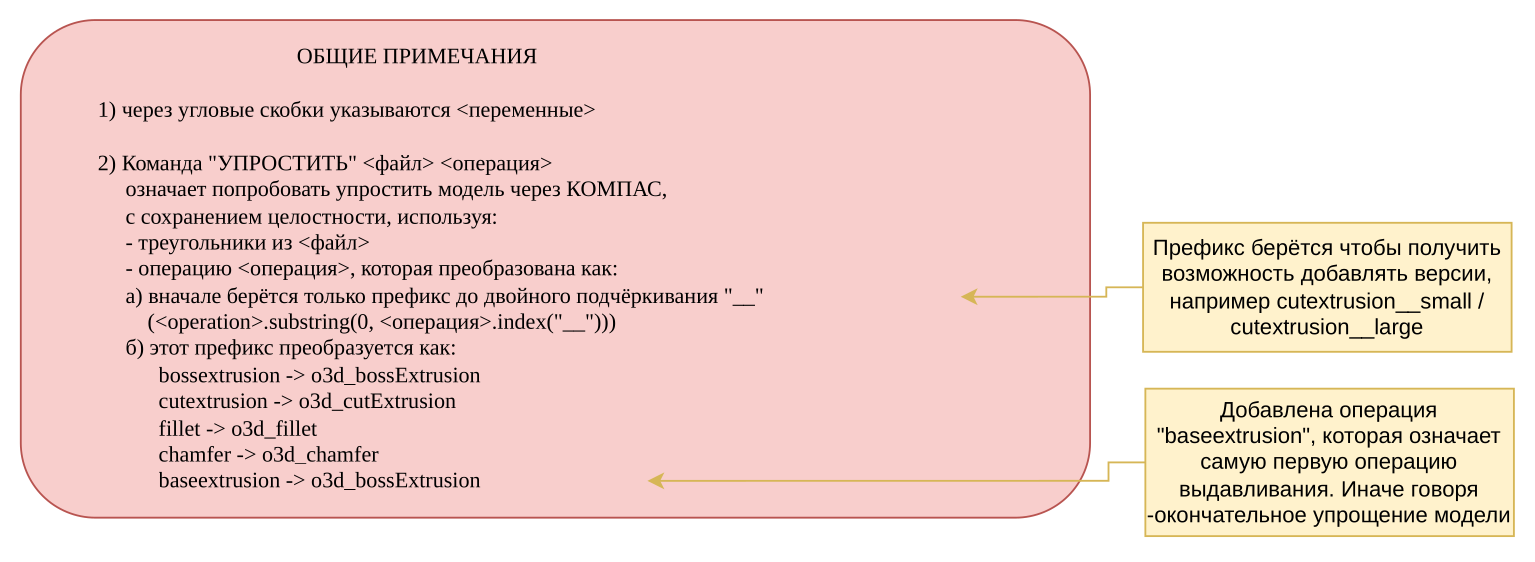
\includegraphics[width=0.5\linewidth]{figures/scheme_general.png}
    \caption{Схема работы main.exe - общее описание}
    \label{fig:placeholder}
\end{figure}

В полуавтоматическом режиме, программе в качестве параметров необходимо указать тип задачи (классификация / сегментация), тип операции, а также опциональные параметры постобработки. В ходе работы происходит препроцессинг исходного файла, вызывается нейронная сеть для выбранных типа задачи и операции, и результат сохраняется в виде файла в указанной папке. Вид файла зависит от типа задачи: в результате классификации получается файл meta.json, в котором указывается поле probability - уверенность нейронной сети в наличии выбранной операции в данной модели; в результате сегментации получается файл test\_0.stl, который содержит геометрию, которая, по мнению нейронной сети, относится к данному типу операции.

\begin{figure}
    \centering
    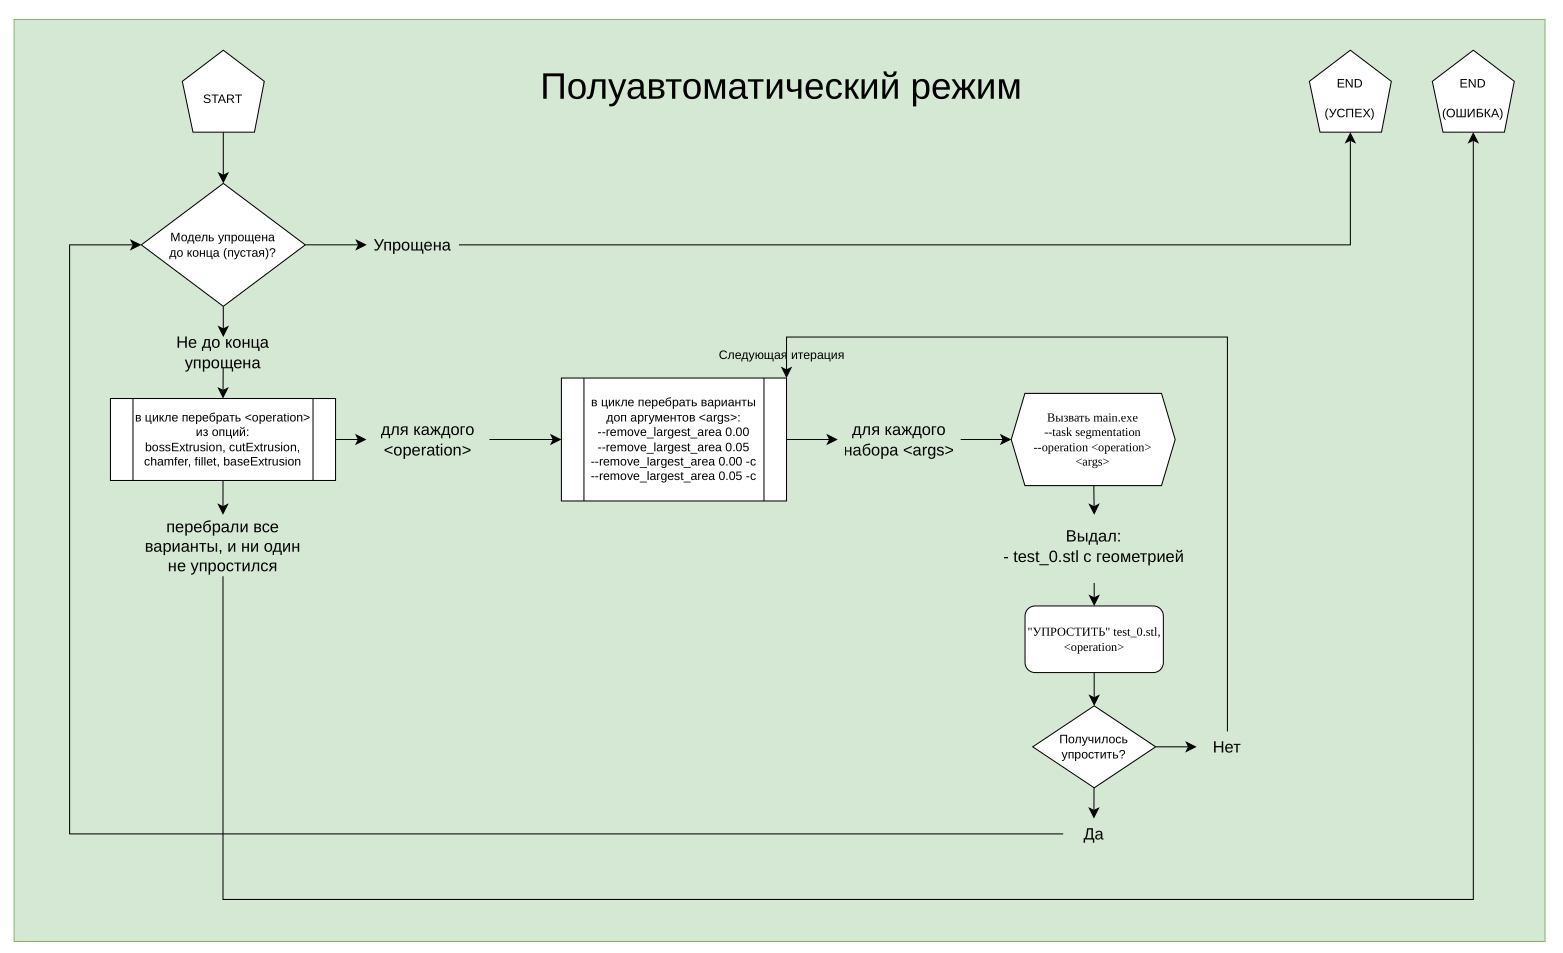
\includegraphics[width=0.5\linewidth]{figures/scheme_mode_semiauto.png}
    \caption{Схема работы main.exe - полуавтоматический режим}
    \label{fig:placeholder}
\end{figure}

В автоматическом режиме, программа получает исключенные из рассмотрения операции, а также опциональные параметры постобработки. В ходе работы она перебирает все доступные ей на данный момент нейронные сети, вызывая вначале классификаторы для каждого типа операции. На основе полученных уровней уверенности в наличии типа операции в модели выбирается тип операции, для которого будет вызвана процедура сегментации. Результатом являются сразу два файла: meta.json, содержащий выбранную операцию и уровень уверенности нейронной сети в наличии этой операции, а также test\_0.stl, который содержит геометрию, которая, по мнению нейронной сети, относится к данному типу операции.

\begin{figure}
    \centering
    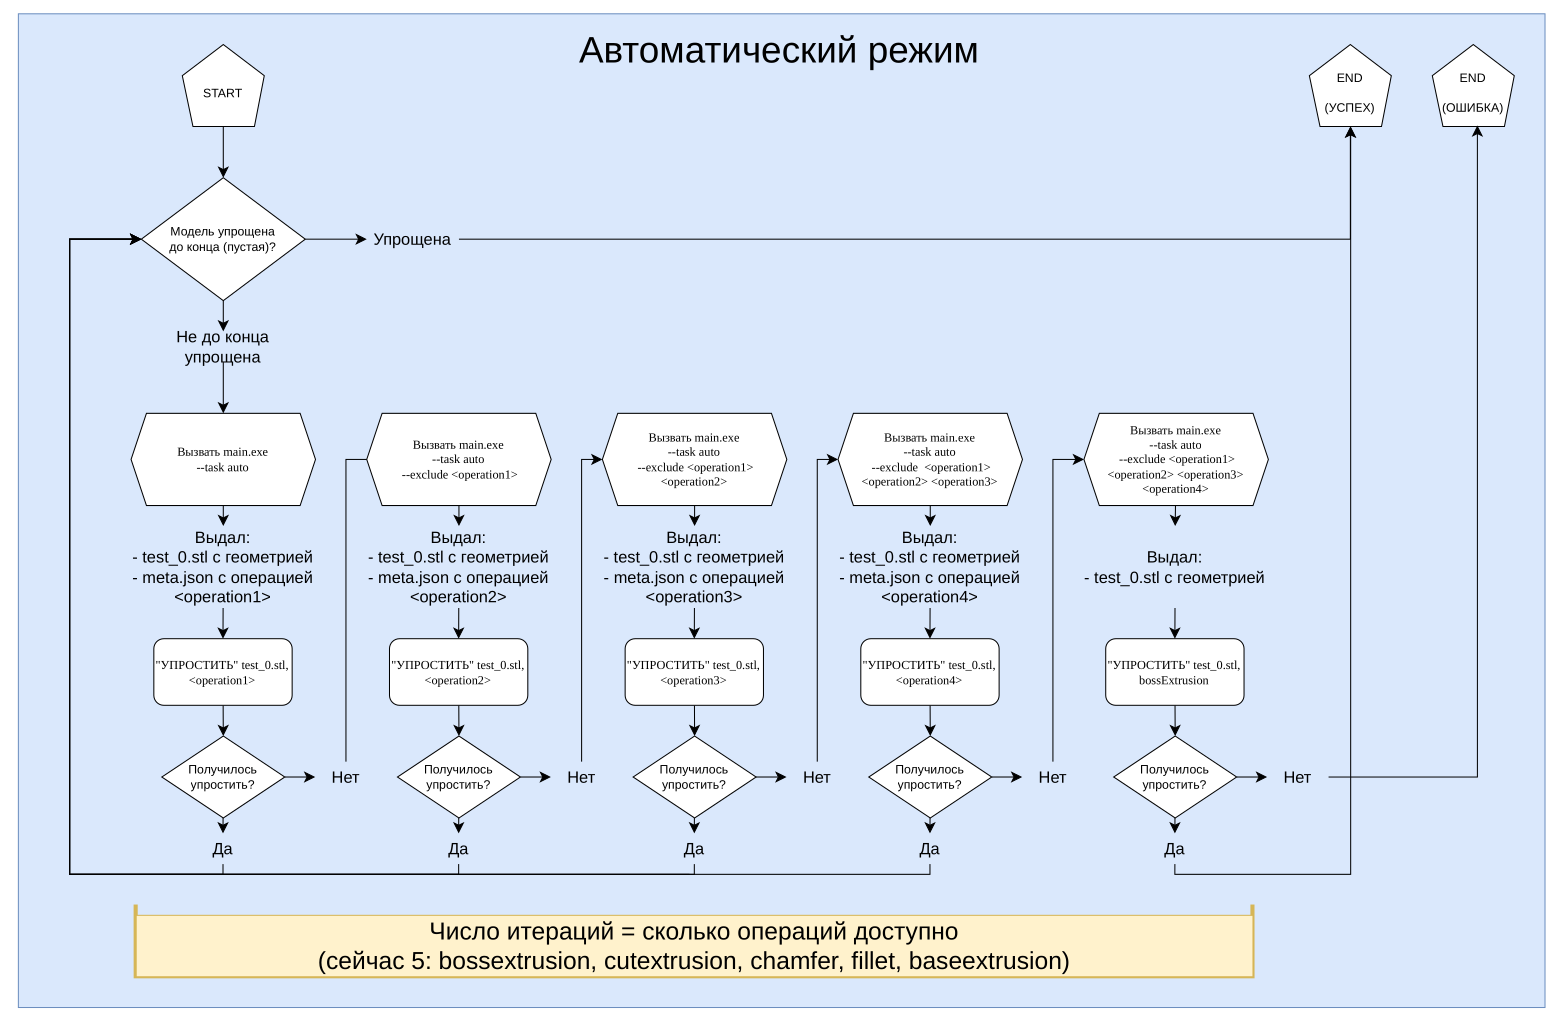
\includegraphics[width=0.5\linewidth]{figures/scheme_mode_auto.png}
    \caption{Схема работы main.exe - автоматический режим}
    \label{fig:placeholder}
\end{figure}

Таким образом, текущий рабочий подход может быть кратко сформулирован как гибридная сегментационно-классификационная схема с детерминированной CAD-постобработкой, мультипредставлением данных и явной интеграцией результатов в прикладной контур КОМПАС-3D.
